% !TeX root = ../thuthesis-caishiyu.tex

\chapter{垃圾回收机制设计}

本章节将从几个设计维度介绍 N2DB 中的垃圾回收机制。
垃圾回收机制既在运行时清理冗余的数据结构,也需要在数据恢复阶段回收泄漏的空间。
因而本文所涉及的垃圾回收可以分为两个场景,一个是运行时,另一个是恢复时。

章节~\ref{sec:gc-goal} 先介绍两个场景的垃圾回收的设计目标。
接着章节~\ref{sec:mvcc} 介绍了存储引擎所使用的并发控制算法。该章节会着重介绍在保证数据结构的崩溃一致性的前提下指令顺序的设计。
之后章节~\ref{sec:space} 会介绍在运行过程以及数据恢复过程中不可见数据的判断方式。
章节~\ref{sec:time} 会解释垃圾回收的时机。
最后章节~\ref{sec:implement} 详细地介绍垃圾回收的流程,以及具体的相关数据结构设计,并且解释了垃圾回收机制如何保证多线程编程的正确性的。


\section{设计目标}
\label{sec:gc-goal}

基于 MVCC 的数据库管理系统在运行时会由于事务的删除操作和更新操作产生不可见的数据结构。
这些数据结构一方面会影响系统的性能,一方面降低存储空间的利用率。
垃圾回收的目的在于如何回收不可见的数据结构。

运行时的垃圾回收的设计目标在于尽可能快且正确地识别以及回收不可见的空间。
由于 N2DB 记录相关的数据结构有 head 以及 version,二者都需要进行可回收判断。
运行时的垃圾回收还需要防止与事务之间的并发冲突以及保证版本链的崩溃一致性。

恢复时的垃圾回收的主要设计目标在于识别并回收内存泄漏的空间。
系统宕机会导致垃圾回收机制中断,
因此恢复时的垃圾回收还需要回收上一次运行时的遗留下的可回收的数据结构。


\section{多版本并发控制算法}
\label{sec:mvcc}
N2DB 采用了多版本并发控制算法。
本章节首先介绍事务开始的流程,之后介绍基于快照的版本可见性判断,接下来介绍了事务在运行时访问版本链的流程,以及读、插入、更新以及删除这 4 个基本操作的流程,最后简单提及事务提交和中止的流程。

\begin{figure}[ht]
    \centering
    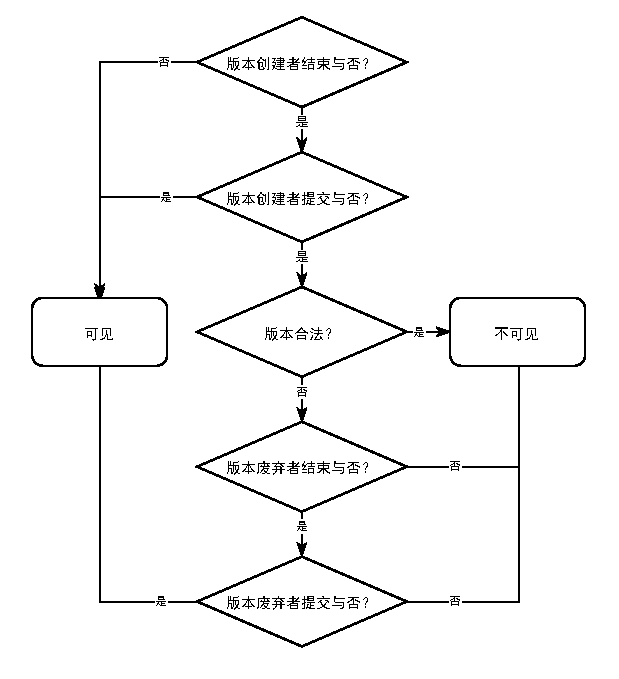
\includegraphics[width=1\linewidth]{figures/version_visibility.pdf}
    \caption{版本可见性的判断流程图}
    \label{fig:version-visibility}
\end{figure}

事务开始时会先申请一个全局唯一的事务 ID。同时事务会获得一个快照 (snapshot)。快照逻辑上是已经结束的事务的集合。已经结束的事务既包括提交的事务也包括中止的事务。根据快照隔离的定义,一个事务只能看到对于自身而言结束的并且提交的事务的影响。

一个记录的版本链存在多个 version。
对于一个事务而言,一个版本链中至多有一个 version 是可见的。
事务通过快照,版本信息以及事务状态数组中的事务信息才能判断这些 version 中哪一个才是对该事务可见的版本。判断的方法称之为版本可见性判断。
图~\ref{fig:version-visibility} 中展示事务的版本可见性判断策略。
版本的可见性判断策略可以分为主要三步:
\begin{enumerate}
    \item 该版本的创建事务已经结束且提交了,否则该版本不可见。
    \item 该版本的 xmax 为正无穷,则说明该版本是可见的。
    \item 该版本被其他事务废弃,然而废弃该版本的事务尚未提交,则该版本是可见的。
\end{enumerate}


% \begin{algorithm}[ht]
%     \caption{事务访问版本链的方法 $access\_version$}
%     \label{alg:traverse_version_chain}
%     \KwIn{The accessed head, $h$\ and the snapshot of the accesser.}
%     \KwOut{Visible version, $v$}
%     \BlankLine
%     \If{ $h$ is empty or $h$ is already deleted}{
%         return $nullptr$;
%     }

%     Set $v$ to the newest version of $h$;

%     \While{ $v$ is not $nullptr$ and $v$ is not visible according to snapshot}{
%         Set $v$ to the older version of $v$;
%     }

%     return $v$;

% \end{algorithm}

事务在运行时有四种基本操作,分别是读,插入,更新以及删除。
同时事务在运行时会将访问过的版本分别记录在四个集合,分别为 read\_set,update\_set,insert\_set 和 remove\_set。事务在读,更新以及删除等操作中,需要访问版本链找到可见的版本。
% 算法~\ref{alg:traverse_version_chain} 中为访问版本链的流程。
事务在访问版本链的过程中会先判断 head 是否合法,即 head 的最新版本不为空且该记录尚未被删除。之后事务会从新到旧遍历所有的版本,直到找到可见的版本。如果找不到可见的版本则会返回空指针。


\textbf{读操作:}对于一个指定的记录,事务首先通过表格的 head\_pages 定位其对应的 head。
之后从该 head 开始遍历版本链,直到找到对于该事务可见的版本。
如果没有找到可见的版本,则说明对于该事务而言,这条记录不存在。

\begin{algorithm}[h]
    \caption{事务的插入操作 $insert$}
    \label{alg:transaction-insert}
    \KwIn{Record data}
    \KwOut{Success or not}
    \BlankLine
    Table allocate a new head, $rh$;

    Table allocate a new version, $rv$;

    Write data into the new version, $rv$;

    \textbf{Fence};

    Modify the newest version of $rh$ to $rv$;

    \textbf{Fence};

    return $true$;

\end{algorithm}

\textbf{插入操作:}算法~\ref{alg:transaction-insert} 为插入操作的流程。首先表格分配一个新的 head 给事务。接下来表格再分配一个新的 version。事务将记录的数据写入新的 version 中,并且写入其他的元数据。
接下来事务使用 fence 指令以保证在写入 head 之前,version 的数据以及元数据已经持久化。
最后事务修改 head 的元数据以及修改 head 的 newest\_version 的指针。
最后事务使用一个 fence 指令保证事务结束该操作时,所有的数据的修改均已持久化。



\textbf{更新操作:}算法~\ref{alg:transaction-update} 为更新操作的流程。事务首先从根据记录 ID 找到对应的 head,之后根据访问版本链的策略得到找到对应的 version。
接下来事务需要判断有没有更新冲突,比如有一个并发的事务在修改同一个记录。
之后表格分配新的 version,事务将记录数据以及其他元数据写入到该 version 中。
然后事务修改可见事务的 xmax ,之后使用 fence 指令保证修改持久化。
最后事务修改 head 的 newest\_version 为新分配的 version 并使用 fence 指令保证上述数据的持久化均已结束。

\begin{algorithm}[h]
    \caption{事务的更新操作 $update$}
    \label{alg:transaction-update}
    \KwIn{Record data and the record id, $rid$}
    \KwOut{Success or not}
    \BlankLine
    Get the record head $rh$ using the record id, $rid$;

    Find the visible version $rv$ using $rh$;

    \If{there is update conflict}{
        return $false$;
    }

    Table allocate a new version, $new\_rv$;

    Write data into the new version, $new\_rv$;

    Modify the $xmax$ of $rv$;

    \textbf{Fence};

    Modify the newest version of $rh$ to $new\_rv$;

    \textbf{Fence};

    return $true$;

\end{algorithm}


\textbf{删除操作:}算法~\ref{alg:transaction-delete} 为删除操作的流程。
事务首先根据记录 ID 在表格中定位对应的 head 的地址。
之后事务找到对于该事务的可见版本 version。
如果该版本为最新版本时,则意味着没有事务冲突。接下来事务更新 head 的 remove\_tx 为该事务的事务 ID,之后使用 fence 指令保证持久化顺序。
如果该版本不是最新版本,则该事务删除操作失败。

\begin{algorithm}[h]
    \caption{事务的删除操作 $delete$}
    \label{alg:transaction-delete}
    \KwIn{The record id, $rid$}
    \KwOut{Success or not}
    \BlankLine
    Get the record head $rh$ using the record id, $rid$;

    Find the version $rv$ using $rh$;

    \eIf{$rv$ is the newset version of $rh$}{
        Modify the $xmax$ of $rv$;

        Modify the $remove\_tx$ of $rh$;

        \textbf{Fence};

        return $true$;
    }{
        return $false$;
    }

\end{algorithm}

\textbf{事务的提交和中止:} 事务在提交和中止时,
会先通过事务状态数组的接口将该事务的状态设置为对应状态。
之后事务会先记录当前已分配的最大事务 ID,max\_seen\_tid。
接下来事务根据自身访问过的记录以及在记录上实施的操作,判断出潜在的可回收的空间。
最后事务将可回收的空间信息与 max\_seen\_tid 一同传递给运行时的垃圾回收组件。
垃圾回收组件会根据这些信息决定回收的时机。


\section{垃圾回收的对象}
\label{sec:space}

本章节将具体地介绍可回收的空间的判断方法。

\subsection{运行时垃圾回收的对象}

事务在运行过程中会根据操作过的版本的信息标记可回收的空间。
当事务提交或者中止后会将可回收的空间信息传递给垃圾回收机制,由垃圾回收机制决定的回收的时机。运行时的可回收的空间根据事务提交或者中止可以分为两大种情况。

\begin{figure}
    \centering
    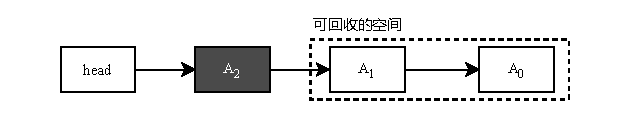
\includegraphics[width=1\linewidth]{figures/gc-a.pdf}
    \caption{提交事务更新操作相关的可回收空间}
    \label{fig:space-commit}
\end{figure}

\begin{figure}
    \centering
    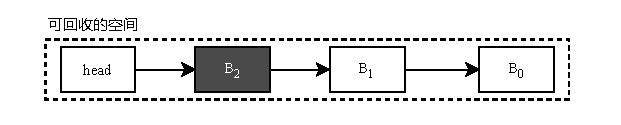
\includegraphics[width=1\linewidth]{figures/gc-b.pdf}
    \caption{提交事务删除操作相关的可回收空间}
    \label{fig:space-commit2}
\end{figure}

首先是提交事务的所标记的可回收空间有两种情况:(1) 当该事务进行更新操作时,会创建一个新的版本。因此当该事务提交之后,比所创建的版本更早的版本可被回收。(2) 事务删除某一条记录并且提交后,该记录所对应的整个版本链是可回收的。

\begin{figure}
    \centering
    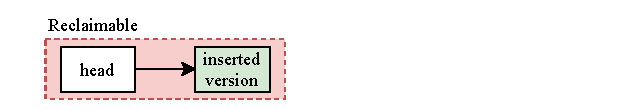
\includegraphics[width=1\linewidth]{figures/gc-c.pdf}
    \caption{中止事务插入操作相关的可回收空间}
    \label{fig:space-abort}
\end{figure}

\begin{figure}
    \centering
    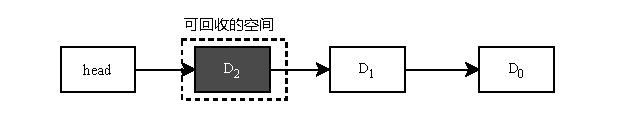
\includegraphics[width=1\linewidth]{figures/gc-d.pdf}
    \caption{中止事务更新操作相关的可回收空间}
    \label{fig:space-abort2}
\end{figure}

其次是中止事务的所标记的可回收空间。如图~\ref{fig:space-abort}所示,同样有两种情况:
(1) 一个事务进行了插入操作,当事务中止之后,因为插入操作所新增的版本链是可以被回收的。(2) 当事务更新了一个记录并且中止之后,所创建的新版本也是不可见的,因此也是可回收的。

\subsection{恢复时垃圾回收的对象}

恢复时的可回收空间可以分为三类:
(1)所有的未分配的 head 以及 version 均是可回收的。
(3)所有不可见的 head 都是可回收的。
(2)版本链中所有不可见的 version。
需要注意的是,未分配的 head 和不可见的 head 是不一样的。未分配指的是该 head 尚未被使用过。
不可见的 head 指的是由于提交事务的删除以及未提交事务的插入导致的 head。


\section{垃圾回收的时机}
\label{sec:time}

本章节将会介绍运行时的四种可回收的空间的回收时机,以及恢复时的可回收空间的回收时机。

\subsection{运行时的可回收空间的回收时机}

事务提交时会将可回收的空间信息传递给垃圾回收机制。
垃圾回收回收机制会在该事务的影响对于所有活跃及所有后续的事务也可见的情况下,对所标记的空间进行回收。
因为当该事务对于全局及后续的事务可见后,所有的后续事务逻辑上永远不会访问到比该事务更新所创建的版本更早的版本。
并且该事务删除记录的影响对全局以及后续事务可见意味着所有事务逻辑上不会访问到被删除的记录。

中止事务的所标记的空间情况相对复杂。
中止事务的影响是对于全局事务永远都不可见的。
因此全局事务不可能访问到中止事务所插入的新的记录,所以插入的新的版本链可以被立刻回收。
中止事务更新所创建的新版本会根据版本可见性原则被所有事务无视。
然而并发的事务在访问版本链的过程中可能会持有该版本的地址。
因此中止事务所创造的新版本不能立刻回收。
中止事务会将此类版本从版本链上断开,如图~\ref{fig:insert-abort} 所示。
直到并发的所有事务均结束后,垃圾回收组件才可能安全地回收该版本。

\begin{figure}
    \centering
    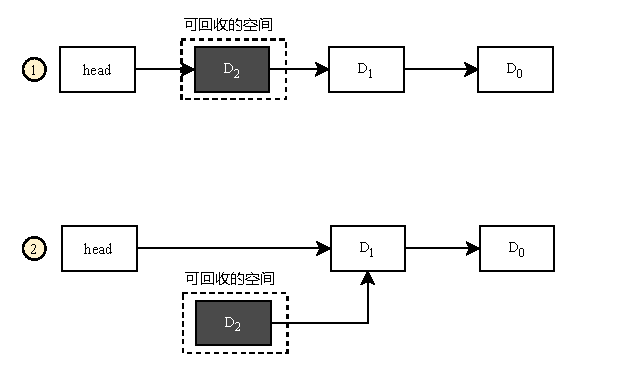
\includegraphics[width=1\linewidth]{figures/gc-e.pdf}
    \caption{事务在中止时对于更新创建的新版本进行的断链操作}
    \label{fig:insert-abort}
\end{figure}

除了中止事务插入的版本链可以立刻被回收外,其他三种情况均需要延后一段时间后才能回收。因此事务会在结束时记录一个时间戳来帮助垃圾回收线程判断回收时机。当事务提交或者中止时,事务会访问全局的事务 ID 的计数器来得到一个最大的已分配的事务 ID,记为 max\_seen\_tid。这三种可回收空间的可回收时机为全局活跃的最小事务 ID 大于 max\_seen\_tid。
对于提交事务而言,当该条件满足时,提交事务的影响对全局可见。
对于中止事务而言,当该条件满足时,并发的事务均已经结束。


\subsection{恢复时的可回收空间的回收时机}

恢复时的可回收空间一共有 3 种情况,分别有不同的回收时机:(1)所有不可见的 head 可以被立刻回收。(2) 版本链中所有不可见的 version 也可以被立刻回收的,也可以由运行时的垃圾回收机制回收。(3)所有未被分配的 version,也就是不在版本链中的 version,需要等到数据恢复机制的后台扫描线程扫描了所有版本链之后才能回收。


\section{系统工程实现}
\label{sec:implement}

本章节会着重介绍在工程实现中的垃圾回收机制设计,包括垃圾回收的频率和粒度、并发冲突的解决以及崩溃一致性的保障。章节~\ref{ssec:gc-metadata} 会先介绍垃圾回收调度器的数据结构定义。然后章节~\ref{ssec:gc-implement} 中展示了事务结束流程中与垃圾回收相关的操作。最后章节~\ref{ssec:gc-implement} 解释垃圾回收调度器的实际的回收操作。

\subsection{垃圾回收调度器的数据结构}
\label{ssec:gc-metadata}


事务在结束阶段会将可回收的空间信息封装成 GCItem,之后将所有 GCItem 传递给垃圾回收机制。
GCItem 中记录了可回收的版本的位置信息。
GCItem 中还需要记录时间戳相关的元数据帮助垃圾回收机制判断回收时机,防止并发的垃圾回收机制对于同一行进行重复回收。
GCItem 的数据结构定义如下:
\begin{itemize}
    \item 表格指针(tbl):表格指针记录了该版本所在的表格的地址。
    \item 事务 ID(tx\_id):事务 ID 为封装该 GCItem 的事务的 ID。
    \item 最大已分配事务 ID(max\_seen\_tid):最大已分配事务 ID 起到帮助垃圾回收调度器判断回收时机的作用。
    \item version 指针(rv):version 指针记录了可回收的版本的地址。
    \item 记录 ID(record\_id):记录 ID 为该版本所对应的记录的标识符。
    \item 垃圾回收时间戳(gc\_ts):垃圾回收时间戳记录该记录的 head 的回收次数,用于防止重复回收。
\end{itemize}

负责进行实际回收操作的组件为垃圾回收调度器(GCScheduler)。
每个线程都一个垃圾回收调度器。
事务在封装完 GCItem 之后会通过调用垃圾回收调度器的 schedule 接口。
该接口会将 GCItem 添加到调度器中的 gc\_items。
垃圾回收调度器的数据结构的定义如下:
\begin{itemize}
    \item 回收队列(gc\_queue):回收队列是一个先进先出(FIFO)的队列,其中每一个元素均为 GCItem。当本线程的事务结束之后,会通过 schedule 接口将封装成 GCItem 的可回收空间添加到该队列中。
    \item 回收阈值(gc\_threshold):回收阈值是一个启动时就已经设定好的参数,用于控制垃圾回收的频率。当回收队列的长度大于回收阈值时,调度器就会开始回收 GCItem 以减少队列的长度。如果回收阈值为 0 时,则意味着每次事务结束时均会触发垃圾回收,系统中的冗余空间会处于一个极低的水平。但是系统频繁地调用垃圾回收会降低系统的性能。在本文的实现中,回收阈值通常为 100。
\end{itemize}



\subsection{事务的提交和中止的流程设计}
\label{ssec:commit-abort}

事务在提交和中止事务的流程中,不仅需要将可回收的空间信息封装 GCItem,同时也会需要进行一些额外操作,比如说回收中止事务插入的版本链和将中止事务更新的新版本移出版本链。本章节将介绍事务提交和中止流程的设计思路以及具体实现。

\begin{algorithm}[h]
    \caption{事务提交的流程}
    \label{alg:commit}
    \BlankLine
    Set transaction status to COMMITTED;

    \ForAll{ accessed versions $rv$ in update\_set}{
        Wrap the previous version of $rv$ into a GCItem; \\
        Append the GCItem into the local queue, gc\_queue;\\
    }

    \ForAll{ accessed version $rv$ in remove\_set}{
        Wrap $rv$ into a GCItem; \\
        Append the GCItem into the local queue, gc\_queue;\\
        Modify $remove\_tx$ of the head;\\
    }

    Record the max\_seen\_tid;

    \ForAll{
        item in gc\_queue
    }{
        Modify item using max\_seen\_tid; \\
        GCScheduler.schedule(item);

    }


\end{algorithm}

\textbf{提交流程:} 如算法~\ref{alg:commit} 所示,事务首先将通过事务状态数组的 set\_status 接口将自身状态设置为 COMMITTED。
接下来对于 update\_set 中的所有版本,将更新所创建的新版本的更老的版本和其他信息封装成 GCItem,添加到事务本地的队列中。
之后对于 remove\_set 中的所有版本,事务将该记录的版本链的最新版本与其他信息封装成 GCItem,然后将其添加到本地队列。
之后事务设置对应 head 的 remove\_tx 为本事务的事务 ID。
在封装两种情况所对应的 GCItem 之后,事务读取全局的事务 ID 计数器,得到当前最大的已分配的事务 ID,max\_seen\_tid。最后事务将本地队列清空,使用 max\_seen\_tid 更新所有 GCItem,之后事务将所有的 GCItem 通过垃圾回收调度器的 schedule 接口传递给调度器。


\begin{algorithm}[h]
    \caption{事务中止的流程}
    \label{alg:abort}
    \BlankLine
    Set transaction status to ABORTED;

    \ForAll{ accessed versions $rv$ in insert\_set}{
        Table reclaims $rv$;
        Table reclaims head of $rv$;
    }

    \ForAll{ accessed version $rv$ in update\_set}{
        Find the head $rh$; \\
        Compare\_and\_swqp($rh.newset\_version$, $rv$, $rv.prev\_version$); \\
        Wrap $rv$ into a GCItem; \\
        Append the GCItem into the local queue, gc\_queue;\\
    }

    Record the max\_seen\_tid;

    \ForAll{
        item in gc\_queue
    }{
        Modify item using max\_seen\_tid; \\
        GCScheduler.schedule(item);

    }


\end{algorithm}

\textbf{中止流程:} 事务中止的流程与事务提交相近,但是更为复杂。首先事务先设置事务状态数组中的自身的状态为 ABORTED。接下来 insert\_set 中的所有版本可以立刻被表格回收。当版本被回收之后,其对应的 head 也可以被表格回收。
之后对于 update\_set 中的所有版本,事务使用一个 CAS 指令原子化修改版本的 head 的 newest\_version 指针,修改成功的话则说明该版本被成功地从版本链上断开。然后事务将 update\_set 中的版本与其他信息封装成 GCItem,将其添加到本地队列中。最后事务记录记录最大的已分配的事务 ID,更新本地队列中所有的 GCItem,最后使用垃圾回收调度器的 schedule 接口传递所有的 GCItem。中止流程中有两个设计要点:

\begin{figure}
    \centering
    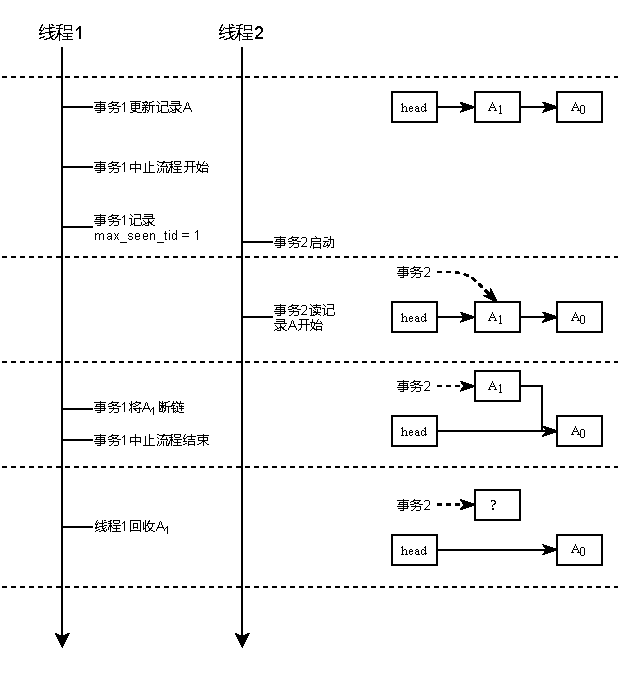
\includegraphics[width=1\linewidth]{read-abort.pdf}
    \caption{事务访问版本链与事务中止流程的并发冲突}
    \label{fig:update-abort-read}
\end{figure}

首先是记录最大的已分配的事务 ID 必须在更新所创建的版本断链之后。假设两者顺序对调,系统会产生故障。
以图~\ref{fig:update-abort-read} 为例,事务 1 中止时记录了最大已分配的事务 ID 为 1。而当事务 1 记录完之后,事务 2 开始了读取记录 A。
事务 2 在读取记录 A 的过程中会物理地持有 $A_1$ 的指针。
之后事务 1 将版本 $A_1$ 从版本链上断开,并结束了中止流程。
该线程的垃圾回收调度器会判断版本 $A_1$ 满足回收条件,并将其回收。
事务 2 此时就会读到异常数据。

\begin{figure}
    \centering
    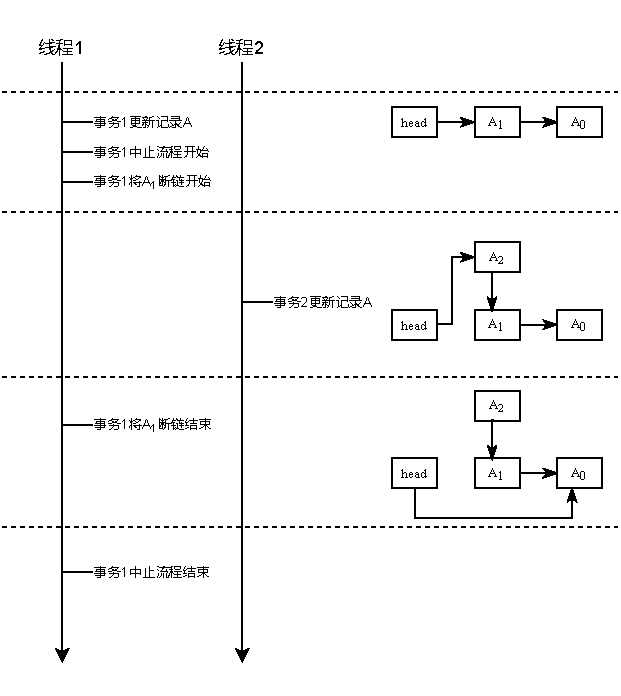
\includegraphics[width=1\linewidth]{update-conflict.pdf}
    \caption{事务更新与事务中止流程的并发冲突}
    \label{fig:update-abort-update}
\end{figure}

其次是通过 CAS 指令修改 head 的 newest\_version 可以无锁地解决并发事务之间的冲突。
假设使用原子写来替换 CAS 指令,会产生事务的更新丢失。
以图~\ref{fig:update-abort-update} 为例,当事务 1 中止之后,事务 2 更新同一条记录 A。
之后事务 2 创建新版本 $A_2$。
事务 1 和事务 2 都需要修改 head 指针,前者需要将指针修改为对应版本的后一个版本,后者则要把指针修改为新分配的版本。
因此如果事务 2 原子性写在前,而事务 1 原子写在后,则事务 2 所创建的新版本 $A_2$ 就不在版本链上。
因此这种情况造成了事务 2 的更新丢失。
而事务 1 在断链操作中使用 CAS 指令可以防止该问题。





\subsection{垃圾回收的流程设计}
\label{ssec:gc-implement}

垃圾回收调度器的回收队列的长度会随着同线程的事务的执行而增加。
当队列长度达到回收阈值之后,垃圾回收调度器就会被触发。
垃圾回收调度会执行 do\_gc 来回收回收队列中的空间。
do\_gc 的具体流程如算法~\ref{alg:do_gc} 所示。

\begin{algorithm}[h]
    \caption{垃圾回收调度器 do\_gc 的流程}
    \label{alg:do_gc}
    \KwIn{The transaction ID of minumum active transaction, $ma\_tid$}
    \BlankLine

    \While{ $gc\_items$ is not empty
    }{
        $item = gc\_items.front()$;\\

        \If{ item.max\_tid > ma\_tid}{
            return;
        }

        \If{
            $item.rv.max == item.rv.min$
        }{
            Table reclaims $item.rv$;\\
            return;
        }

        \If{$item.rh.gc\_ts != item.gc\_ts$} {
            return;
        }

        Lock the version chain;

        \For{
            version $v$ in the version chain
        }{
            \If{ $v == item.rv$
            }{
                Find the newer version of $item.rv$;

                Spilt the version chain on $item.rv$;
            }
        }

        Unlock the version chain;

        Table reclaims all version in remaining chain;

        \If{
            $item.rh.newset\_version == nullptr$
        }{
            Update $item.rh.gc\_ts$;

            Table reclaim $item.rh$;
        }

        gc\_items.pop();
    }


\end{algorithm}


首先垃圾回收调度器获取全局活跃的最小事务 ID,记为 ma\_tid。当 gc\_items 的中的
GCItem 满足其 max\_seen\_tid 小于 ma\_tid 时,则调度器可以回收该 GCItem 对应的空间。

接下来调度器需要判断 GCItem 的类型。在章节~\ref{sec:space} 中,不能立刻回收的空间有三种:一是提交事务的更新操作对应的空间,二是提交事务的删除操作所对应的空间,三是中止事务的更新操作所对应的空间。当调度器判断 GCItem 属于第三种情况时,则调度器会立即回收 GCItem 所对应的版本,并且结束回收工作。

由于每个线程均有一个垃圾回收调度器,一个版本链上的空间可能会被重复回收。
因此调度器需要根据 head 中的 gc\_ts 判断该 head 对应的版本链是否已经被回收过了。如果 head 已经被回收了,
调度器就直接结束该 GCItem 的回收工作。

调度器从 head 开始从新到旧访问版本链。
在访问版本链之前,调度器对于该记录进行加锁以防止并发的调度器和事务对于该版本链进行指针操作。
如果没有找到 GCItem 所对应的版本,则意味着该版本已经被其他调度器回收了,因此调度器释放锁并且结束回收工作。
如果调度器找到对应的版本,则通过一个原子写修改对应版本的更新版本的后向指针,将 GCItem 所对应的版本及后面所有更老的版本从版本链上断开,之后调度器释放锁。

调度器从断开的版本链从新到旧依次回收所有的版本。

在版本回收工作结束之后,如果 head 之后已经没有版本,则意味着该行是被删除了。之后调度器自增 head 的 gc\_ts,以防止其他调度器重复回收该记录。
最后该 head 被回收。

至此调度器对一个 GCItem 的回收工作结束。
调度器接着判断 gc\_items 中下一个 GCItem 满不满足回收条件,若满足则重复此过程。


\section{本章小结}

本章节从设计目标,并发控制,回收对象,回收时机这四个方面介绍了 N2DB 中的垃圾回收机制的设计思路,之后从系统实现角度详细地介绍垃圾回收的具体流程。

首先,垃圾回收机制的设计目标在于回收存储引擎中不可见的空间,以提高存储空间利用率。
由于 N2DB 是多版本的数据存储结构,垃圾回收机制涉及了两种记录相关的数据结构 head 以及 version。

其次,由于垃圾回收机制与事务的并发控制算法紧密耦合,章节~\ref{sec:mvcc} 中大致介绍了事务的运行时协议以及四个基本操作的流程。

接下来章节~\ref{sec:space} 在并发控制算法的基础上介绍了垃圾回收机制对于可回收的空间的判断标准。
对于运行时的垃圾回收机制而言,可回收的空间可以根据事务提交与否和操作类型分为四类情况。
对于恢复时的垃圾回收机制而言,可回收的空间可以分为三种,分别是上一轮运行过程所遗留下来的未被回收的空间,尚未分配的空间和分配但未被使用的空间。

然后章节~\ref{sec:time} 介绍了运行时的四种可回收空间以及恢复时的三种可回收空间的回收时机。
运行时的四种可回收空间中有一种可以在事务结束时立刻回收,而剩下三种需要延后一段时间才能在不影响后续事务的运行的前提下回收。
恢复时的可回收空间可以分为三种情况,不可见的 head 需要被立刻回收,而剩下两种情况可以延后。

最后章节~\ref{sec:implement} 介绍了运行时的垃圾回收机制的实现。每个线程都有一个负责垃圾回收的垃圾回收调度器。事务执行结束后会将可回收的空间信息封装成 GCItem 传递给调度器。
之后调度器在满足条件的情况下回收对应的 GCItem。
由于垃圾回收组件与别的线程的事务和垃圾回收组件是并发执行的,因此本章节着重解释了并发冲突的解决方法。
